\begin{figure}[h!]
	\centering
	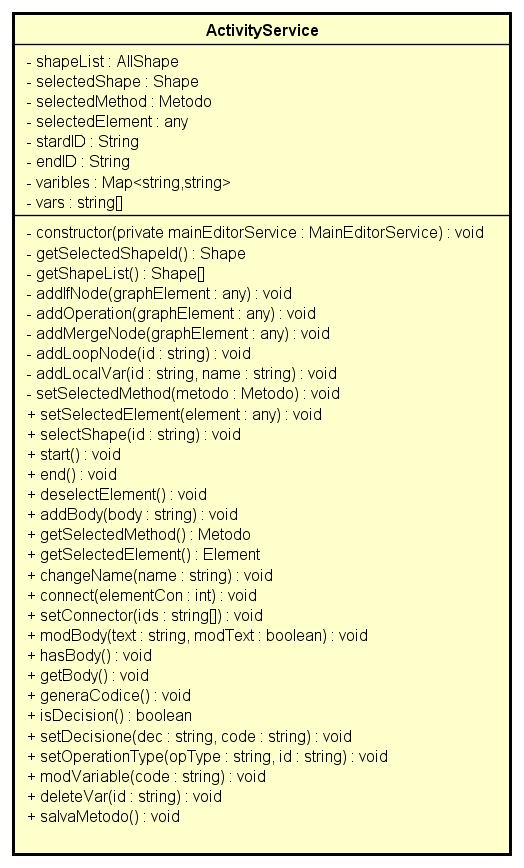
\includegraphics[scale=0.8]{res/sections/SpecificaFrontEnd/Services/Disegnetti/activity.png}
	\caption{Diagramma della classe ActivityService}
\end{figure}

\begin{itemize}
	\item \textbf{Descrizione:}\\
	
	\item \textbf{Utilizzo:}\\
	
	\item \textbf{Attributi:}
		\begin{itemize}
			\item \emph{-shapeList:AllShape}\\
			
			\item \emph{-selectedShape: Shape}\\
			
			\item \emph{-selectedMethod: Metodo}\\
			
			\item \emph{-selectedElement: any}\\
			
			\item \emph{-stardID: string}\\
			
			\item \emph{-endID: string}\\
			
			\item \emph{-varibles: Map<string, string>}\\
			
			\item \emph{-vars: string[]}\\
			
		\end{itemize}
	\item \textbf{Metodi:}
		\begin{itemize}
			\item \emph{-constructor(private mainEditorService: MainEditorService}\\
    		\\
    		\textbf{Parametri:}
    		\begin{itemize}
    			\item \emph{mainEditorService: MainEditorService}\\
    			
    		\end{itemize}
    		\item \emph{-getSelectedShapeId()}\\
    		
    		\item \emph{-getShapeList()}\\
    		
    		
    		\item \emph{-addIfNode(graphElement: any)}\\
    		\\
    		\textbf{Parametri:}
    		\begin{itemize}
    			\item \emph{graphElement: any}\\
    			
    		\end{itemize}
    		\item \emph{-addOperation(graphElement: any)}\\
    		\\
    		\textbf{Parametri:}
    		\begin{itemize}
    			\item \emph{graphElement: any}\\
    			
    		\end{itemize}
    		\item \emph{-addMergeNode(graphElement: any)}\\
    		\\
    		\textbf{Parametri:}
    		\begin{itemize}
    			\item \emph{graphElement: any}\\
    			
    		\end{itemize}
    		\item \emph{-addLoopNode(id: string)}\\
    		\\
    		\textbf{Parametri:}
    		\begin{itemize}
    			\item \emph{id: string}\\
    			
    		\end{itemize}
    		\item \emph{-addLocalVar(id: string, name: string)}\\
    		\\
    		\textbf{Parametri:}
    		\begin{itemize}
    			\item \emph{id: string}\\
    			
    			\item \emph{name: string}\\
    			
    		\end{itemize}
    		\item \emph{-setSelectedMethod(metodo: Metodo)}\\
    		\\
    		\textbf{Parametri:}
    		\begin{itemize}
    			\item \emph{metodo: Metodo}\\
    			
    		\end{itemize}
    		\item \emph{+setSelectedElement(element: any)}\\
    		\\
    		\textbf{Parametri:}
    		\begin{itemize}
    			\item \emph{element: any}\\
    			
    		\end{itemize}
    		\item \emph{+selectShape(id: string)}\\
    		\\
    		\textbf{Parametri:}
    		\begin{itemize}
    			\item \emph{id: string}\\
    			
    		\end{itemize}
    		\item \emph{+start()}\\
    		
    		\item \emph{+end()}\\
    		
    		\item \emph{+deselectElement()}\\
    		
    		\item \emph{+addBody(body: string)}\\
    		\\
    		\textbf{Parametri:}
    		\begin{itemize}
    			\item \emph{body: string}\\
    			
    		\end{itemize}
    		\item \emph{+getSelectedMethod()}\\
    		
    		\item \emph{+getSelectedElement()}\\
    		
    		\item \emph{+getNameMethod()}\\
    		
    		\item \emph{+getVarVis()}\\
    		
    		\item \emph{+getShapeType()}\\
    		
    		\item \emph{+changeName(name:string)}\\
    		\\
    		\textbf{Parametri:}
    		\begin{itemize}
    			\item \emph{name: string}\\
    			
    		\end{itemize}
    		\item \emph{+connect(elementCon)}\\
    		\\
    		\textbf{Parametri:}
    		\begin{itemize}
    			\item \emph{elementCon: any}\\
    			
    		\end{itemize}
    		\item \emph{+setConnector(ids: string[])}\\
    		\\
    		\textbf{Parametri:}
    		\begin{itemize}
    			\item \emph{ids: string[]}\\
    			
    		\end{itemize}
    		\item \emph{+modBody(text: string, modText: boolean)}\\
    		\\
    		\textbf{Parametri:}
    		\begin{itemize}
    			\item \emph{text: string}\\
    			
    			\item \emph{modText: boolean}\\
    			
    		\end{itemize}
    		\item \emph{+hasBody()}\\
    		
    		\item \emph{+getBody()}\\
    		
    		\item \emph{+generaCodice()}\\
    		
    		\item \emph{+isDecision()}\\
    		
    		\item \emph{+isVarDeclaration()}\\
    		
    		\item \emph{+setDecisione(dec: string, code: string)}\\
    		\\
    		\textbf{Parametri:}
    		\begin{itemize}
    			\item \emph{dec: string}\\
    			
    			\item \emph{code: string}\\
    			
    		\end{itemize}
    		\item \emph{+setOperationType(opType: string, id: string)}\\
    		\\
    		\textbf{Parametri:}
    		\begin{itemize}
    			\item \emph{opType: string}\\
    			
    			\item \emph{id: string}\\
    			
    		\end{itemize}
    		\item \emph{+modVariable(code: string)}\\
    		\\
    		\textbf{Parametri:}
    		\begin{itemize}
    			\item \emph{code: string}\\
    			
    		\end{itemize}
    		\item \emph{+deleteVar(id: string)}\\
    		\\
    		\textbf{Parametri:}
    		\begin{itemize}
    			\item \emph{id: string}\\
    			
    		\end{itemize}
    		\item \emph{+salvaMetodo()}\\
    		
		\end{itemize}
\end{itemize}